\chapter{Features Interpretation}

    Once features have been extracted by the way of some techniques described in the previous chapter one need to interpret these features in order to achieve end applications. What I mean by interpret is that based on the features one of the following questions, depending on the problem at hand, has to be answered : \say{Can we identify an object in the Image ?}, \say{What is the class of the image ?}, \say{Are these two image similar ?} \ldots

    \section{Similarity Measure}

    An obvious objective in CBIR is to assess the similarity of a query image with images in database. Different similarity measure have been investigated for this. Also algorithms that are able to learn a similarity measure from training data have been developed. The choice of the right metric to use is of course dependent of the problem at hand but also of the technique that was used to extract the features. Indeed depending on which techniques was used the representation of the image will differ. In the survey of Datta and all \cite{datta2008image} they call these different representations signatures and they discern between three types of signature :

    \begin{description}
      \item[Single Vector] The image is represented as a single features vector. It is for instance the result of using a global shape descriptor.

      \item[Set of Vectors] The image is represented as a set of vectors and is usually the result of features computed on different regions obtained by segmentation of the image.

      \item[Histogram] The image is represented as an histogram. This can be the result of the shallow methods introduced previously.

    \end{description}

      \subsection{Fixed Measure}

      Basic metrics for computing the similarity between two features vectors include the minkowski distance or the cosine similarity. However when computed based on low-level features such metrics often fail to concur the distance computed and the semantic similarity. An attractive measure for measuring the distance between two probability distribution is the Earth Mover Distance (EMD) introduce by Rubner and all in 2000 \cite{rubner2000earth}. The EMD is based on the minimal cost that must be paid to transform one distribution into the other and matches perceptual similarity better than other distances. Another metric is the Kullback–Leibler Distance used for instance by Do and all \cite{do2002wavelet} to compute the similarity from waveket-based texture features.

      \subsection{Similarity Learning}

        Rather that using a fixed measure learning another approach is to rely on machine learning to learn a similarity measure. Three common setups exist :

        \begin{description}
          \item[Regression similarity learning] In this approach pairs of image are given \( (I_i^1, I_i^2 ) \) with their associated measure of similarity \( y_i \) and the goal is to learn a function that approximate \( f(I_i^1, I_i^2)  = y_i \).

          \item[Classification similarity learning] In this approach pairs of image are given \( (I_i^1, I_i^2 ) \) with binary labels \( y_i \in \{0, 1\} \). The goal is to learn a classifier able to judge new pairs of images.

          \item[Ranking similarity learning] This time training samples consist to triplet \( (I_i, I_i^+, I_i^-) \) where \( I_i \) is know to be more similar to \( I_i^+\) than to  \( I_i^-\).

        \end{description}

        An example of ranking similarity learning for large scale image learning is the OASIS algorithm \cite{chechik2010large} that model the similarity function as a bilinear form : Given two images \( I_1 and I_2 \) the similarity is measured through the form \( I_1*W*I_2 \) where matrix W is not required to be positive or symmetric.

    \section{Ontology}

    Object Ontology can be used to map low-level features to high level entities. An illustration of an object ontology is show by the figure \ref{ontology}. With this example a concept such as sky could be defined as having a blue color, a upper position and an uniform texture. This way by extracting color, texture and other features from an images different regions can be mapped to concepts. Object ontology is used by Hyvonen and all \cite{hyvonen2003ontology} to access pictures of the promotional events of the university of Helsinki. Top-level ontological categories represent concepts such as Persons, Events, Places and pictures are mapped to theses entities when inserted into the database. In the work by Mezaris and all \cite{mezaris2003ontologies} the images are first segmented then color and shape descriptors are extracted enabling the mapping of each regions to a corresponding concept.

    \begin{figure}[H]
      \centering
        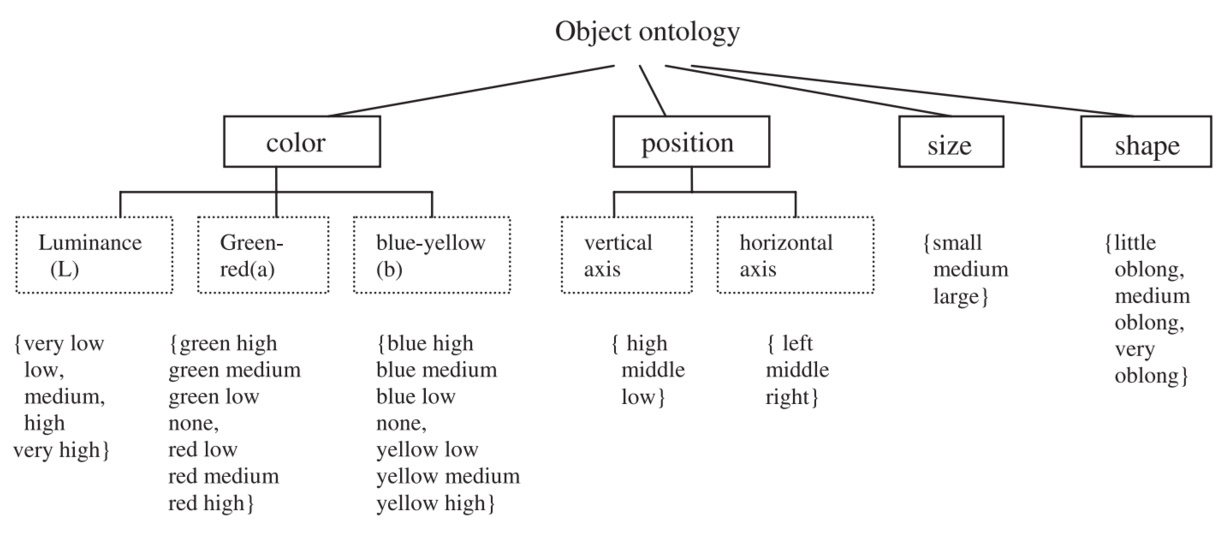
\includegraphics[width=1\textwidth]{images/ontology.png}
        \caption{Object Ontology}
        \label{ontology}
    \end{figure}

    \section{Machine Learning}

    A last approach to associate features with high-level concept is to rely on supervised learning methods. A good candidate which has proven to show strong performance is the support vector machine (SVM) classifier. SVM has originally been designed for binary classification so that we need to train multiple models if we want to achieve multi-classification. The idea behind SVM is to find a hyperplane that best divide the features belonging to two separate classes. Among the possible hyperplane a common one is the \textit{optimal separating plane} which maximize the distance between the hyper-plane and the nearest data point of each class. SVM has often been used in conjunction with the Visual Bag-Of-Word representation to classify images. This is the case for example for the work of Csurka and all \cite{csurka2004visual} or the one of Lowe and all \cite{lowe2004distinctive}.
    Another common classifier is the naive bayes classifier. It relies on the baye's theorem so that prior probabilities and class-conditional densities for the features have to be computed from the training sample. In the work of Vailaya and all \cite{vailaya2001image} they use first and second order moments in the LUV color space as color features and MSAR texture features. Then they perform vector quantization with the learning vector quantization (LVQ) algorithm and the result is fed as input to the naive bayes classifier. This scheme is used to classify indoor / outdoor and city / landscape image. Other classifier that have been investigate are neural network and decision trees.
